% !TEX TS-program = pdflatex
% !TEX encoding = UTF-8 Unicode
% !BIB TS-program = biber
% !BIB program = biber

\documentclass[11pt]{article}

%%% PAGE DIMENSIONS
\usepackage[margin=2.00cm]{geometry}
\geometry{a4paper} 
% \usepackage{caption}
% \usepackage{subcaption}
\usepackage{graphicx} % For better graphics
\usepackage{pdfpages} % To insert pdfs into the library
\usepackage{tikz}
\usepackage{wrapfig}
\usepackage{siunitx}
% Packages to add projects
\usepackage{movie15}
\usepackage{qtree}
% Display multiplication and division sums
\usepackage{xlop}
\usepackage{longdivision}


%%% PACKAGES
\usepackage{booktabs} % for much better looking tables
\usepackage{amsmath} % for better maths
\usepackage{paralist} % very flexible & customisable lists (eg. enumerate/itemize, etc.)
\usepackage{verbatim} % adds environment for commenting out blocks of text & for better verbatim
\usepackage{subfig} % make it possible to include more than one captioned figure/table in a single float
\usepackage[framed,numbered]{matlab-prettifier} % enable inserting matlab code.
\usepackage[parfill]{parskip}
%\addtolength{\jot}{1em}
\usepackage{amssymb}
\usepackage{cancel}
\usepackage{color}
\usepackage{listings}
% Create Listing Colours
\usepackage{xcolor}
% Create directory structures
\usepackage{dirtree}
% Control linespacing
\usepackage{lipsum}
\usepackage{setspace}
\setstretch{0.5}
\usepackage{lscape}
% \definecolor{codegreen}{RGB}{0,255,0}
% \definecolor{codegray}{RGB}{105,105,105}
% \definecolor{codepurple}{RGB}{138,43,226}
% \definecolor{backcolour}{RGB}{255,255,255}
\definecolor{codegreen}{rgb}{0,0.6,0}
\definecolor{codegray}{rgb}{0.5,0.5,0.5}
\definecolor{codepurple}{rgb}{0.58,0,0.82}
\definecolor{backcolour}{rgb}{0.95,0.95,0.92}

\lstdefinestyle{mystyle}{
    backgroundcolor=\color{backcolour},   
    commentstyle=\color{codegreen},
    keywordstyle=\color{magenta},
    numberstyle=\tiny\color{codegray},
    stringstyle=\color{codepurple},
    basicstyle=\ttfamily\footnotesize,
    breakatwhitespace=false,         
    breaklines=true,                 
    captionpos=b,                    
    keepspaces=true,                 
    numbers=left,                    
    numbersep=5pt,                  
    showspaces=false,                
    showstringspaces=false,
    showtabs=false,                  
    tabsize=2
}
\lstset{style=mystyle}

\usepackage{multicol}
\usepackage{float}

% References
\usepackage[backend=biber,style = apa]{biblatex}
\bibliography{sources}

%%% HEADERS & FOOTERS
\usepackage{fancyhdr} % This should be set AFTER setting up the page geometry
\setlength{\headheight}{15pt}
\pagestyle{fancy} % options: empty , plain , fancy
\renewcommand{\headrulewidth}{0pt} % customise the layout...
\lhead{FINANCE 751}\chead{Assignment 1}\rhead{Connor McDowall \& Ben Crosland}
\lfoot{}\cfoot{\thepage}\rfoot{}

%%% SECTION TITLE APPEARANCE
\usepackage{sectsty}

%%% ToC (table of contents) APPEARANCE
\usepackage[nottoc,notlof,notlot]{tocbibind} % Put the bibliography in the ToC
\usepackage[titles,subfigure]{tocloft} % Alter the style of the Table of Contents
\renewcommand{\cftsecfont}{\rmfamily\mdseries\upshape}
\renewcommand{\cftsecpagefont}{\rmfamily\mdseries\upshape} % No bold!

%%% Hyperlinking 
\usepackage{hyperref}
\begin{document}
\section{FINANCE 751 Technical Note}
This technical note informs software installation, transcript extraction, implementation and comparison methodologies to ascertain measures of corporate culture in NZX50 companies, and six Australian commercial banks, using 258 earnings call transcripts. 
This note describes the steps taken to implement Option-2, replicating the corporate culture results.
Additionally, this technical note is for a MacOS operating system and assumes basic proficiency in package management and Python programming. 
\subsection{Installation}
This section informs the installation of required software to facilitate analysis.
\begin{enumerate}
    \item Install several software packages to run the StanfordCoreNLP to measure corporate culture from text files and develop transcript processing code. 
    \hyperlink{https://www.anaconda.com/}{Anaconda} is a distribution of the Python programming language, simplifying package management to develop code in the Python language.
    \hyperlink{https://code.visualstudio.com/}{Microsoft Visual Studio Code} is an integrated development environment, suitable for application building.
    The combination of both Anaconda and Microsoft Visual Studio Code enable programming environments to process the transcripts.
    \item Secondly, clone the remote \hyperlink{https://github.com/MS20190155/Measuring-Corporate-Culture-Using-Machine-Learning}{repository} implementing the method described by Li et al., (\citeyear{li2021measuring}) to your local directory.
    Read the instructions carefully for correct installation.
    In particular, change the \textbf{os.environ ["CORENLP\_HOME"]} variable in \textbf{global\_options.py} file to the installation location of the \textbf{stanford-corenlp-full-2018-10-05} directory on your local device.
    Install the required python packages excluded from Anaconda using the pip package and requirements.txt with the \textbf{pip install requirement.txt} command in the terminal.
    Some packages require specific versions. If you need to revert to a previous version, use the terminal command \textbf{pip install PackageName==Version} to revert to a previous version.
    \item Test the correct installation of the StanfordCoreNLP using the document text files from remote repository by following the ReadMe instructions. 
    Progress to transcript extraction after the successful execution of the StanfordCoreNLP. Otherwise, review the above installation process before progressing.
\end{enumerate} 
\subsection{Transcript Extraction}
This section informs extracting earnings call transcripts from Capital IQ.
\begin{enumerate}
    \item Review the firm\_id column in the 1.firm\_score.xlsx sheet from Option-1 to identify the companies related to the 258 earnings call transcripts.
    \item Navigate to \hyperlink{https://www.capitaliq.com/}{Capital IQ}, selecting the companies tab, followed by the transcripts link.
    \item In the search criteria company search bar, type in and select each of the unique companies listed in the firm\_id column mentioned above.
    The selected entities will update to list sixteen companies as Telecom Corp of New Zealand Ltd changed rebranded to Spark new Zealand Limited.
    \item Change the time frame from 01/01/2009 to 01/10/2021 to ensure you include all 258 transcripts listed in the 1.firm\_score.xlsx spreadsheet and select search in middle-right of the webpage.
    \item Select all transcripts on the page by ticking the top tick box middle-left of the webpage.
    \item Click the options dropbox middle-left of the webpage, and select Download in .Zip file to download all selected documents into a .Zip file.
    \item Scroll to the bottom of the page to select the next subset of transcripts.
    \item Repeat steps five through seven to downloaded all transcripts in .Zip files.
    \item Create a new local directory titled 'transcripts', unzip all .Zip files, moving all transcripts to this newly created directory.
    \item Review the transcripts in the 'transcripts' directory. The filenames align with the filename column in the 1.firm\_score.xlsx spreadsheet. 
    There will be multiple transcripts with the same name e.g., Air New Zealand Limited - ShareholderAnalyst Call.pdf. 
    Consult filename and calltime columns in 1.firm\_score.xlsx to identify the correct transcripts according to date e.g., 201510 is October 2015 , deleting the incorrect duplicates.
    After, the subset of 258 transcripts will exist amongst the full set in the transcript directory.
\end{enumerate}
\subsection{Implementation}
This section highlights the code to process earnings call transcripts, execute the StanfordCoreNLP and compare the results.
The implementation was partitioned into three Python functions within the finance-751-cmcd398.py script (\ref{code}).
This section provides a high level overview of the code with further details described in the code comments.
Transcripts have a common structure. The first three pages are front-matter. The last page is the legal disclaimer.
Some transcripts don't have Q\&A sections while others have multiple. 
The transcripts without Q\&A sections are isolated and excluded during processing.
Transcripts with multiple Q\&A sections are manually condensed prior to processing but excluded during comparison.
\subsubsection{Variables}
The definition of several variables and arrays take place prior to implementation.
\begin{enumerate}
    \item Set strings describing the relative paths for the 1.firm\_score.xlsx file, transcript directory, selected transcript directory to move 258 transcripts of interest, transcript directory for processed transcripts after removing Q\&A sections,
    documents.txt file, documents\_ids.txt, and processed text directory.
    \item Review each transcript in the 1.firm\_score.xlsx filename column to record the page number for the first page of the Q\&A section, appending each value to the end of an array.
    If no Q\&A section exists, record a value of 4. \textbf{The preservation of order is imperative with the position of the page number matching the position of the filename in the filename list from 1.firm\_score.xlsx}.
    \item Set an array listing the set of company ids from the 1.firm\_score.xlsx spreadsheet aligning with an array listing the cumulative position of the final transcript corresponding to the company id.
    For example, Air New Zealand (ANZ) has 11 transcripts. Auckland International Airport (AIA) has 13 transcripts. Therefore, ANZ and AIA have values of 11 and 24, respectively, in the cumulative position array. 
    \item Set strings describing the relative paths for output files, results spreadsheet, and firm scores outputs from the StanfordCoreNLP.
    \item Set binary variables (TRUE or FALSE) to control the execution of the below functions.
\end{enumerate}
\subsubsection{Prepare\_documents.py}
This function isolates the Q\&A sections of each transcript, converts each transcript to a line in a text file, and returns the document text file and identification.
The following sequence of functions are nested within, called on in the order below.
\begin{enumerate}
    \item \textbf{get\_transcripts} extracts a list of filenames from the 1.firm\_score.xlsx spreadsheet, transferring transcripts of interest to the transcripts selected directory.
    \item \textbf{remove\_transcript\_metadata} deploys the pdfrw package to extract each page of the Q\&A section per transcript, using the array denoting the starting page number for the Q\&A section, creating a processed transcript stored in the transcripts processed directory.   
    \item \textbf{create\_ids} creates various forms of identification in data frames for comparison while excluding transcripts without Q\&A sections.
    \item \textbf{create\_documents\_text} deploys the pdfminer package to convert each processed transcript into a single line of text, appending each line to the document.txt file to use as an input for the StanfordCoreNLP.
\end{enumerate}
\subsubsection{Perform\_stanford\_nlp.py}
This function executes each one of the five Python functions integral to StanfordCoreNLP in the following order.
The provision of two separate dictionaries (NZD/AUS and US) informs analysis.
\begin{enumerate}
    \item \textbf{parse.py} to parse the raw documents.
    \item \textbf{clean\_and\_train.py} to clean, remove stopwords, and named entities in the parsed documents text file.
    \item \textbf{create\_dict.py} to create the expanded dictionary.
    \item \textbf{score.py} to score the document. This implementation uses the TF-IDF weights used in the article.
    \item \textbf{aggregate\_firms.py} to aggregate the scores to the firm-time level.
\end{enumerate}
Complete steps one, two and three.
Next, replace the expanded\_dictionary.csv in the dict directory with the AUS/NZD trained dictionary. 
It is possible to manually edit these dictionaries in attempts to improve scores. 
However, the provided dictionaries trained to ascertain the original scores. 
Therefore, the provided dictionaries were left unchanged in replicating scores.
Next, Run score.py and aggregate\_firms.py, saving the scores\_TFIDF.csv as an xlsx file to the comparisons directory. 
Repeat steps four and five with the US dictionary.
\subsubsection{Compare\_results.py}
This function combines a formatted 1.firm\_scores.xlsx document with the TF-IDF output scores from perform\_stanford\_nlp.py by merging data frames on document identification in order to make comparisons.
Compare\_results.py must be repeated for both dictionaries.
After, combine both comparison spreadsheets to compare results from both sets of dictionaries, deleting duplicate values.
\subsection{Comparison}
This section compares our replication of the measures for corporate culture across the five values (Innovation, Integrity, Quality, Respect, Teamwork) using NZ/AUS and US dictionaries. 
We acknowledge the provided scores have slightly shorter document lengths, likely from different pdf to text conversion methodologies.
Our analysis detected a few abnormalities in the aforementioned subset of transcripts, omitting the majority of Q\&A sections (\ref{MQA}), in addition to a subset of transcripts not including Q\&A sections but trained on presentation sections.
The author's emphasize the presentation sections in transcripts are likely not a true reflection of company culture as edited by corporate lawyers and PR personal. 
Subsequently, we exclude these transactions during processing.
\subsubsection{Accuracy Measures}
Absolute and percentage differences between our replication and the provided results are displayed in the 751-comparison.xlsx workbook.
However, we utilize the following equations to measure the accuracy of our replication across companies, values, and total results.
\begin{multicols}{2}
    \begin{equation}
        \text{Individual} = 1-\frac{\sum_{i}|\text{New}_{i,j,k} - \text{Old}_{i,j,k}|}{\sum_{i}\text{Old}_{i,j,k}} \space \forall j,k
    \end{equation}\break
    \begin{equation}
        \text{Total} = 1-\frac{\sum_{i}\sum_{j}\sum_{k}|\text{New}_{i,j,k} - \text{Old}_{i,j,k}|}{\sum_{i}\sum_{j}\sum_{k}\text{Old}_{i,j,k}}
    \end{equation}
\end{multicols}
\begin{multicols}{2}
    \begin{equation}
        \text{Company} = 1-\frac{\sum_{i}\sum_{k}|\text{New}_{i,j,k} - \text{Old}_{i,j,k}|}{\sum_{i}\sum_{k}\text{Old}_{i,j,k}} \space \forall j
    \end{equation}\break
    \begin{equation}
        \text{Value} = 1-\frac{\sum_{i}\sum_{j}|\text{New}_{i,j,k} - \text{Old}_{i,j,k}|}{\sum_{i}\sum_{j}\text{Old}_{i,j,k}} \space \forall k
    \end{equation}
\end{multicols}
\begin{align}
    i &\epsilon \{1,...,N\}\\
    j &\epsilon \{\text{Air New Zealand,...,Westpac Banking Corporation}\}\\
    k &\epsilon \{\text{Innovation,Integrity, Quality, Respect, Teamwork}\}
\end{align}
\subsubsection{Results}
\textbf{Individual}, \textbf{Company}, \textbf{Value}, and \textbf{Total} measure the accuracy of our replication for a specific company and value, company across all values, value across all companies, and across all values and companies respectively.
The accuracy results are displayed in a matrix (\ref{RM}). There are a few abnormalities. The value Teamwork for Goodman Property Trust is NA as both values in the original results are zero. 
Our replication for Teamwork using the NZD/AUS dictionary, and Respect using the US dictionary, deviate relatively from provided figures in our replication.
The later driven by material differences in Infratil's replication (-89\%) and 80\% accuracy for Westpac Banking Corporation.
The remaining results from the Respect value using the US dictionary are above \~80\%.
However, all Teamwork results using the NZD/AUS dictionary are above 83\%, not raising cause for concern.
The \textbf{Company} level of accuracy is above 90\% for all Company IDs.
Each \textbf{Value} level of accuracy is above 90\% except for the Respect value measured by the US dictionary (\~80\%). Finally, the \textbf{Total} level of accuracy is 93\%.
Discrepancies may be caused by small differences in documents lengths, or abnormalities when parsing documents using StanfordCoreNLP.
In summary, our results are highly accurate and satisfactory across Company IDs and Values, providing supporting evidence our replication is successful.
\newpage
\printbibliography
\subsection{Appendix}
\subsubsection{Transcripts with Multiple Q\&A Sections} \label{MQA}
The following transcripts have multiple Q\&A sections.
The sections are consolidated into one section by deleting the presentation material in between the Q\&A sections.
However, they are excluded from comparison calculation as Helen only uses the last Q\&A section.
We took the perspective the last section alone does not proxy for the entire Q\&A sections in the transcript. Therefore, not suitable for measuring corporate culture given the document lengths.
\begin{itemize}
    \item Australia and New Zealand Banking Group Limited - ShareholderAnalyst Call.pdf, 
    \item Bank of Queensland Ltd. - ShareholderAnalyst Call.pdf
    \item Commonwealth Bank of Australia - ShareholderAnalyst Call.pdf
    \item Infratil Limited - AnalystInvestor Day.pdf
    \item Infratil Ltd. - AnalystInvestor Day.pdf
    \item National Australia Bank Limited - ShareholderAnalyst Call.pdf
\end{itemize}
\begin{landscape}
\subsubsection{Result Matrix}\label{RM}
\begin{figure}[h]
    \centering
    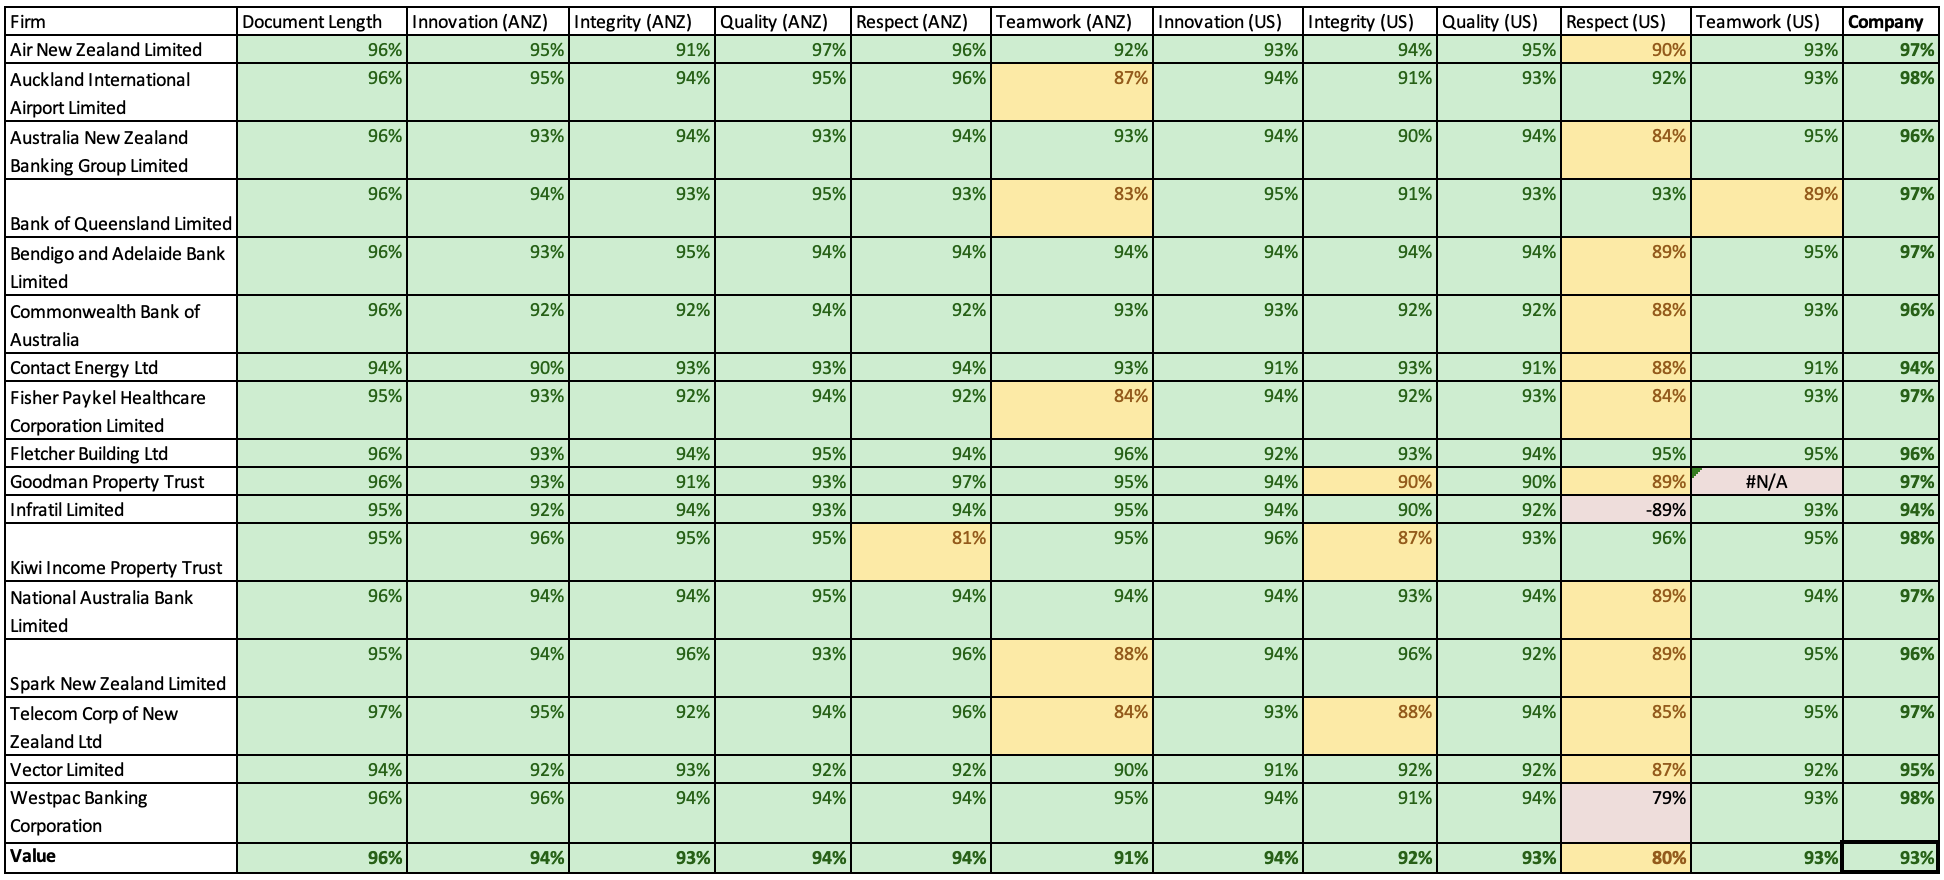
\includegraphics[width=1.5\textwidth]{RM.png}
    \caption{Results Matrix}
    \label{fig:mesh1}
\end{figure}
\end{landscape}
\subsubsection{Python}\label{code}
\lstinputlisting[language=Python]{finance-751-cmcd398.py}
\end{document}